\documentclass{beamer}
\usepackage{graphicx, subfigure}

\usetheme[compress]{Dresden}
\setbeamertemplate{navigation symbols}{} 

\title{Locate My Plate \\ A License Plate Localisation System}
\subtitle{presented by: Tjerk Kostelijk, Folkert Huizinga}
\date{July 1, 2009}

\begin{document}

\frame{\titlepage}

\setcounter{tocdepth}{1}

\frame
{
  \frametitle{Outline}
  \small
  \tableofcontents
  \normalsize
}

\setcounter{tocdepth}{2}

\AtBeginSection[]
{
 \begin{frame}
  \frametitle{Outline}
  \small
  \tableofcontents[currentsection,hideothersubsections]
  \normalsize
 \end{frame}
}

% TODO introduction
\section{Introduction}
\frame
{
  \frametitle{Introduction}
	
  \begin{itemize}
  \item <+-| alert@+> Implementation License Plate Localisation
  \item <+-| alert@+> Feature Analysis
  \item <+-| alert@+> Cascading Classifier
  \item <+-| alert@+> Strong Classifier
  \item <+-| alert@+> Weak Classifier
  \end{itemize}
}

\section{Features}
\frame
{
  \frametitle{What is a feature}
	
	% TODO vertical feature
  \begin{itemize}
	% maybe you rember from computer vision class image filter
  \item <+-| alert@+> Image Filter/scanning window
  \item <+-| alert@+> Properties
		\begin{itemize}
			\item <+-| alert@+> Blocks with sign 
			\item <+-| alert@+> Orientation: Horizontal or Vertical
			\item <+-| alert@+> Image type: 1st/2nd order derivative in x/y direction
			% TODO derrivative images
		\end{itemize}
  \item <+-| alert@+> Feature value
	%Pixels under featureblock are added up/substracted 
  %Gives feature a value for every position in the image
  \end{itemize}
}

\frame
{
	\begin{figure}[!ht]
		\centering
		\subfigure{
		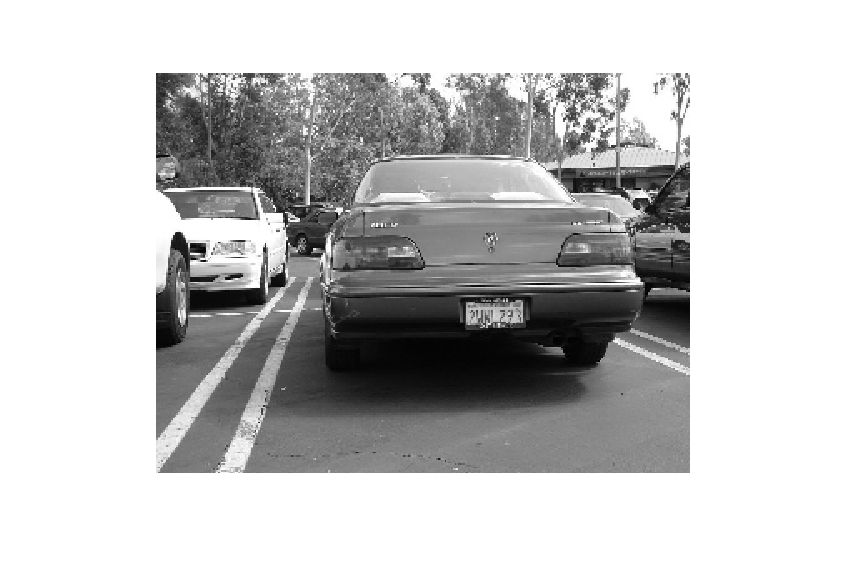
\includegraphics[height=3.5cm]{../report/img/original}
		\label{fig:a}
		}
		\subfigure{
		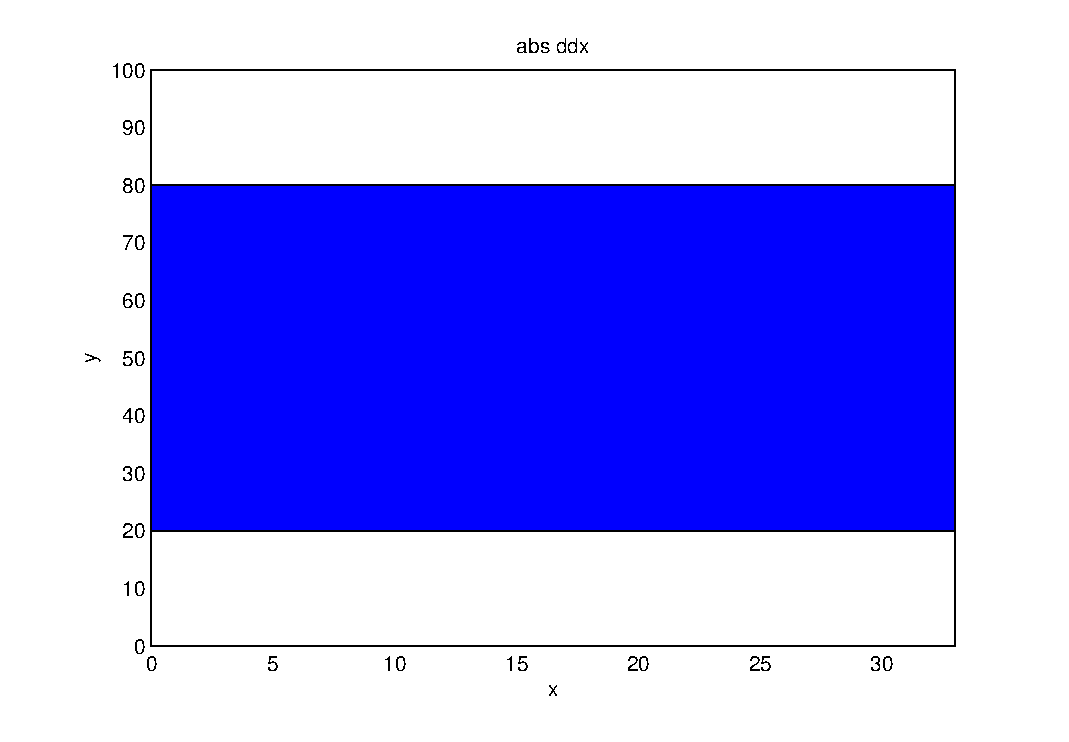
\includegraphics[height=3.5cm]{../report/img/feature}
		\label{fig:b}
		}
		\subfigure{
		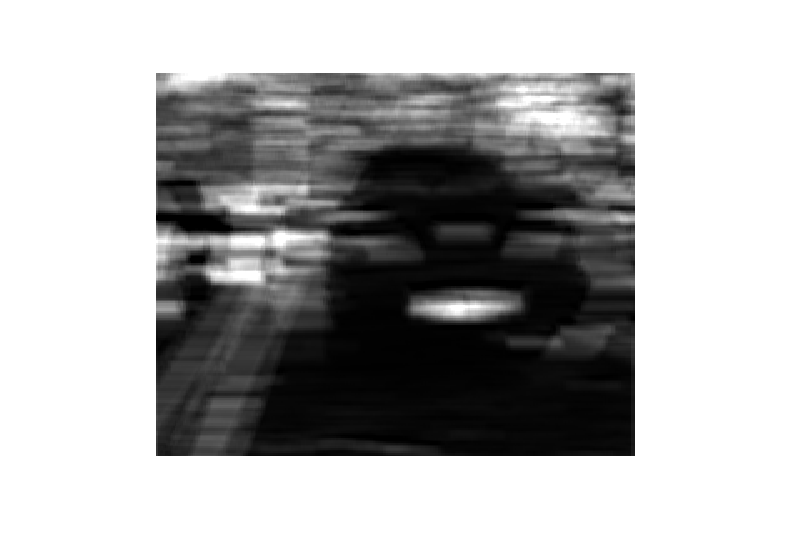
\includegraphics[height=3.5cm]{../report/img/featureapplied}
		\label{fig:c}
		}
		\label{fig:feature}
	\end{figure}
}

\frame
{
  \frametitle{Feature generation}
	% TODO feature
	\begin{itemize}
		\item <+-| alert@+> Feature as binary string
		% position is featureblock, sign is addition/substraction
		\item <+-| alert@+> Generate all possible permutations
		\item <+-| alert@+> Remove inverse one's (101 = 010)
	\end{itemize}
	% TODO table 0001 00010 000011
}

\section{Stage I: Weak}

\frame
{
  \frametitle{What is a weak classifier}
	%Classifies for every point in a image if it contains a license plate
	\begin{itemize}
		\item <+-| alert@+> Properties
			\begin{itemize}
				\item <+-| alert@+> Feature
				\item <+-| alert@+> Threshold
				\item <+-| alert@+> Operator $<$ or $>$
			\end{itemize}
		\item <+-| alert@+> Returns a binary image
	\end{itemize}
	 %The locations of the ones in B correspond to the location of possible license plates.
}
\frame
{
  \frametitle{Training the weak classifier}
	\begin{itemize}
		\item <+-| alert@+> How to learn the threshold and operator $<$ or $>$
		\item <+-| alert@+> Sort on value
		\item <+-| alert@+> Find optimal separation (threshold)
		\item <+-| alert@+> 00001000011111110111111
		\item <+-| alert@+> 000010000-11111110111111
	\end{itemize}
}

% TODO dataset
\section{Stage II: Strong}
\frame
{
  \frametitle{Stage II: Strong}
	
  \begin{itemize}
  \item <+-| alert@+> xxx
  \end{itemize}
}

\frame
{
	\begin{figure}[!ht]
	\centering
	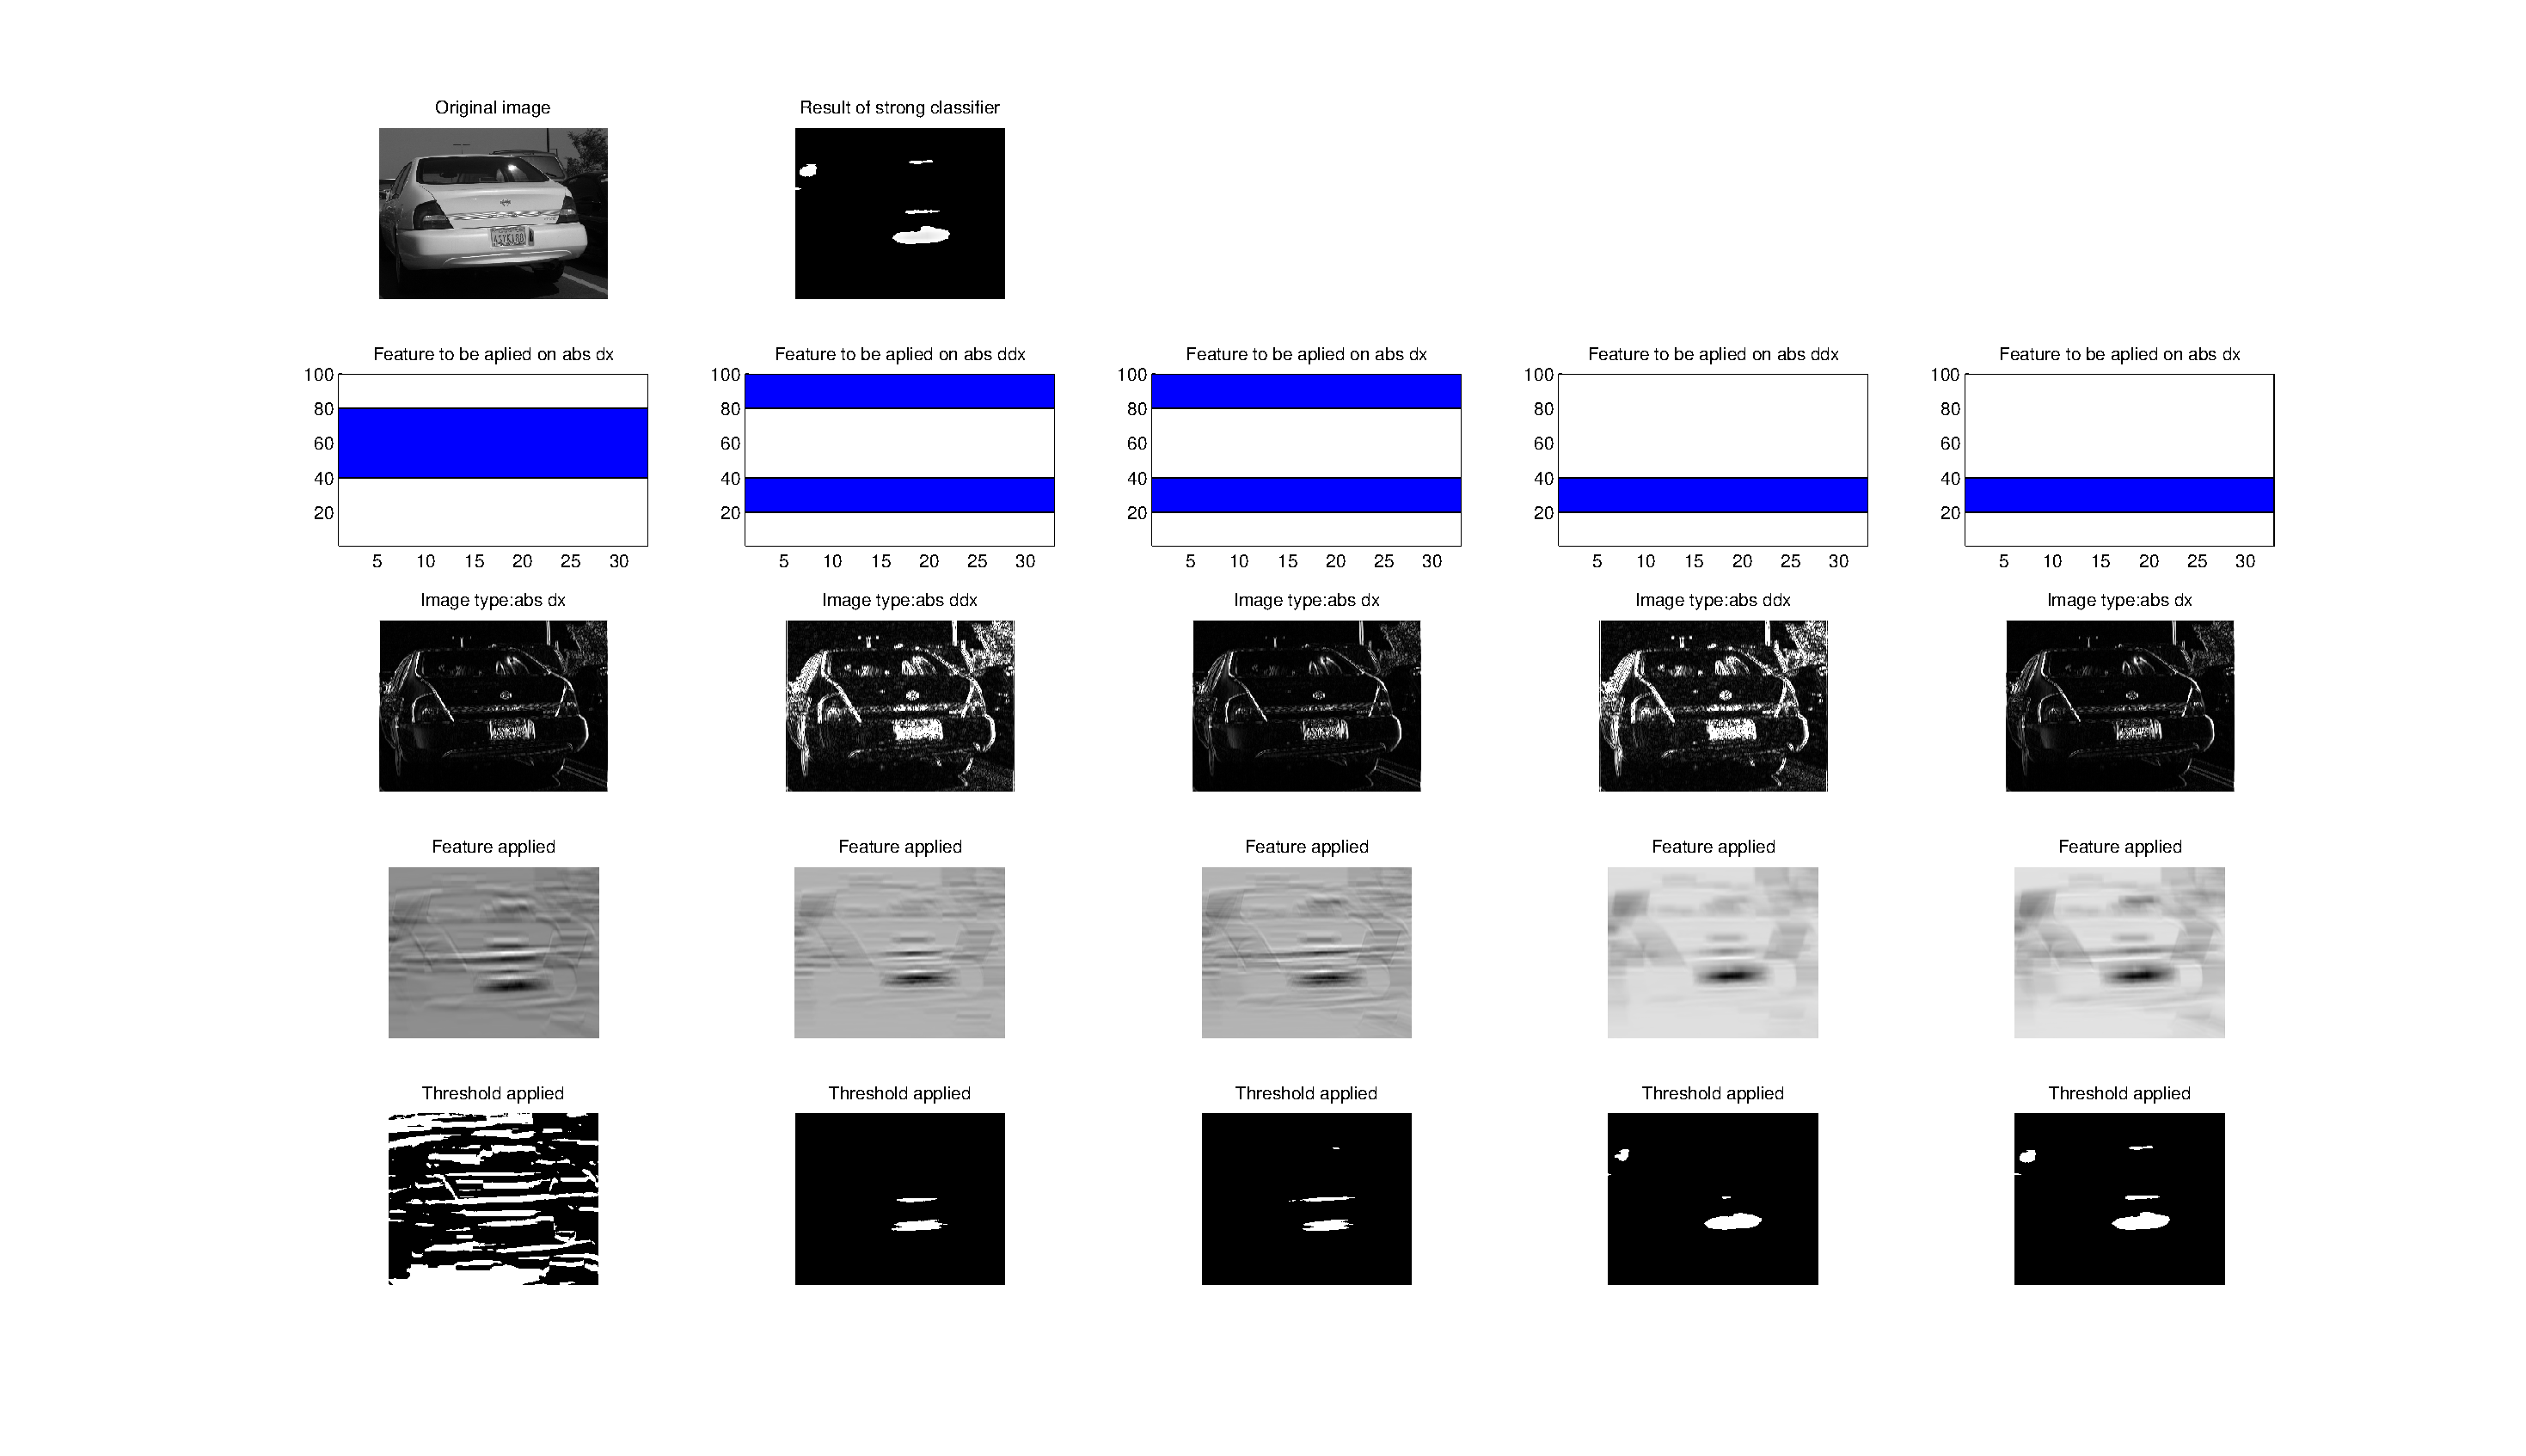
\includegraphics[width=10cm]{../report/img/strongClassifier_layer2_img14}
	\label{fig:strongclassify}
	\end{figure}
}

\section{Stage III: Cascading}
\frame
{
  \frametitle{Stage III: Cascading}
	
  \begin{itemize}
  \item <+-| alert@+> xxx
  \end{itemize}
}

\frame
{
	\begin{figure}[!ht]
	\centering
	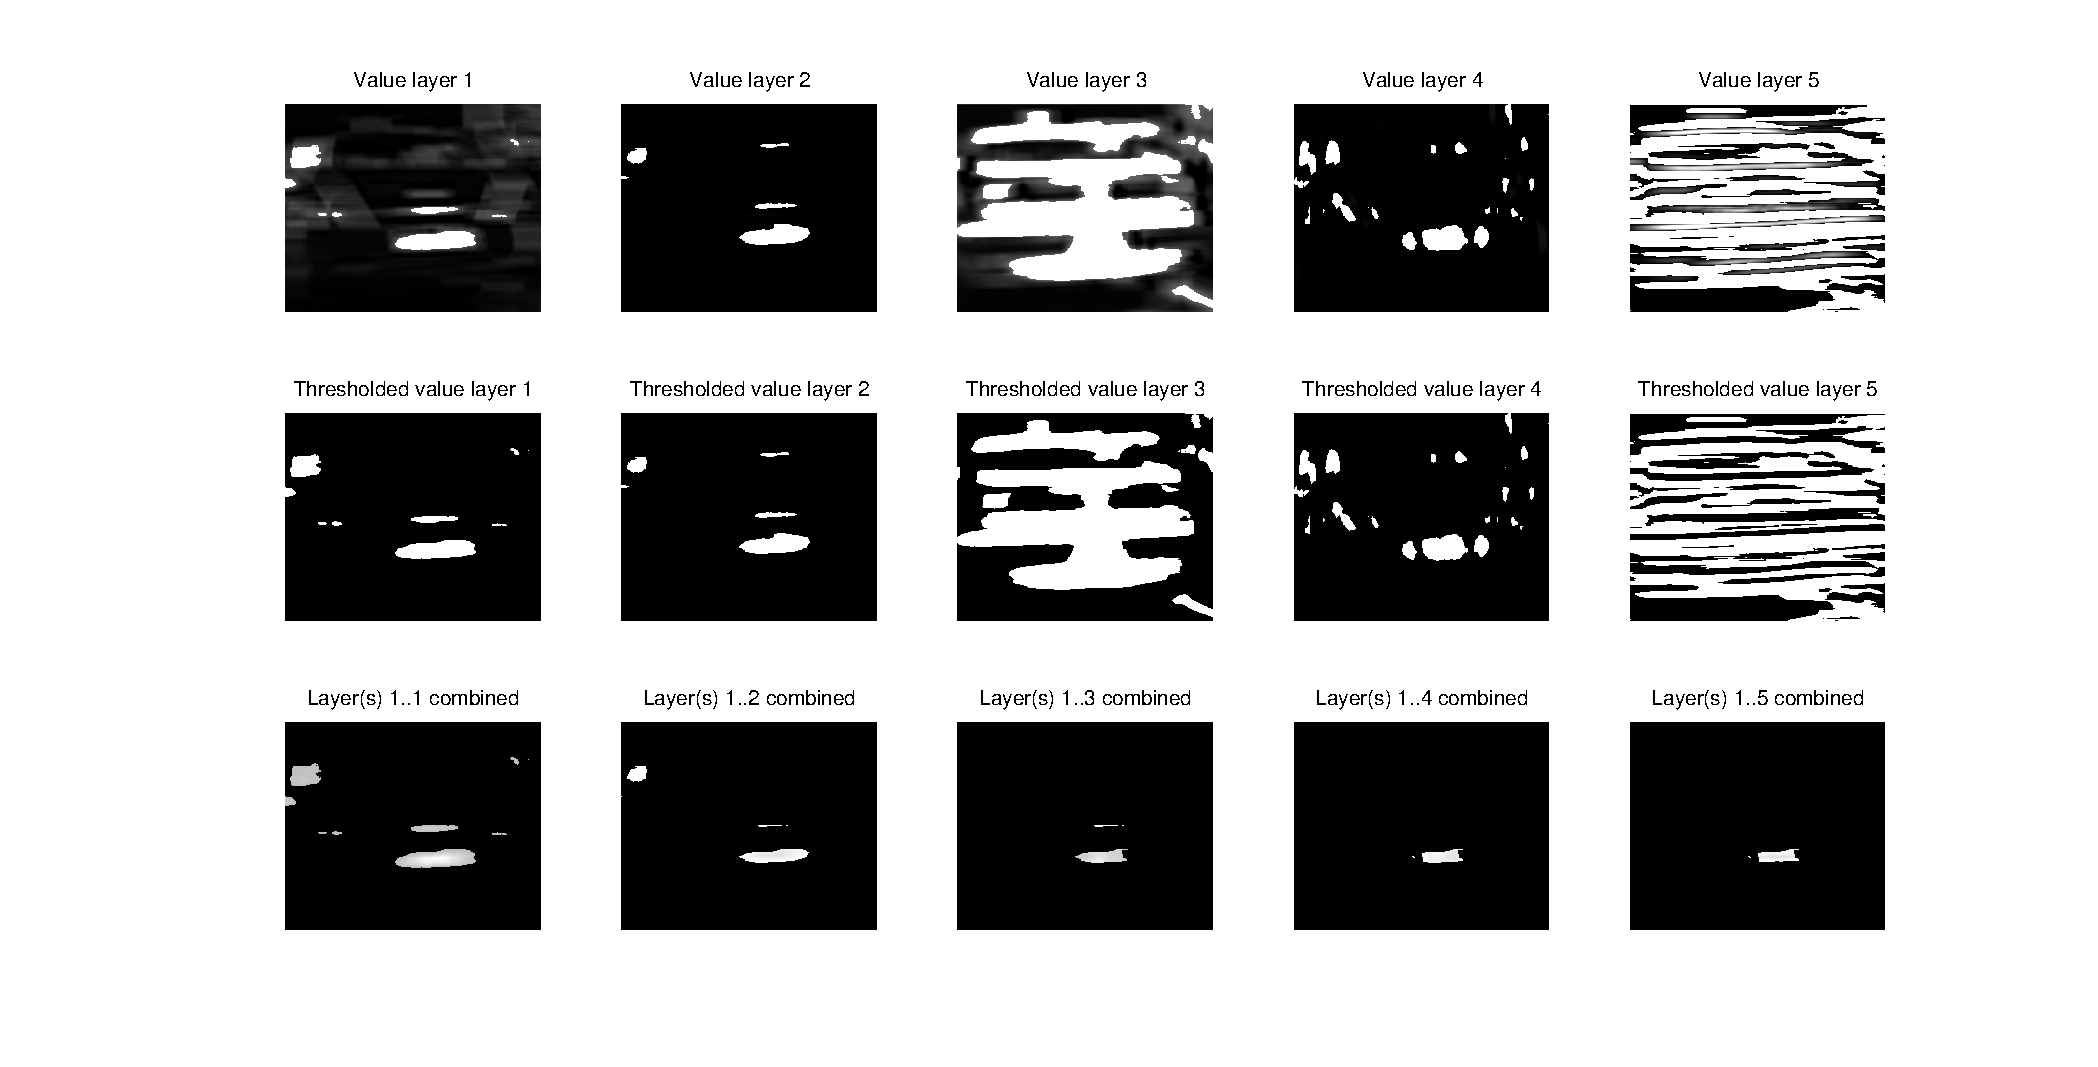
\includegraphics[width=12cm]{../report/img/cascader_img14}
	\label{fig:cascader}
	\end{figure}
}

\section{Results}
\frame
{
  \frametitle{Results}
	
  \begin{itemize}
  \item <+-| alert@+> xxx
  \end{itemize}
}

\frame
{
  \frametitle{Results}
	\begin{figure}[!ht]
	\centering

		\subfigure{
			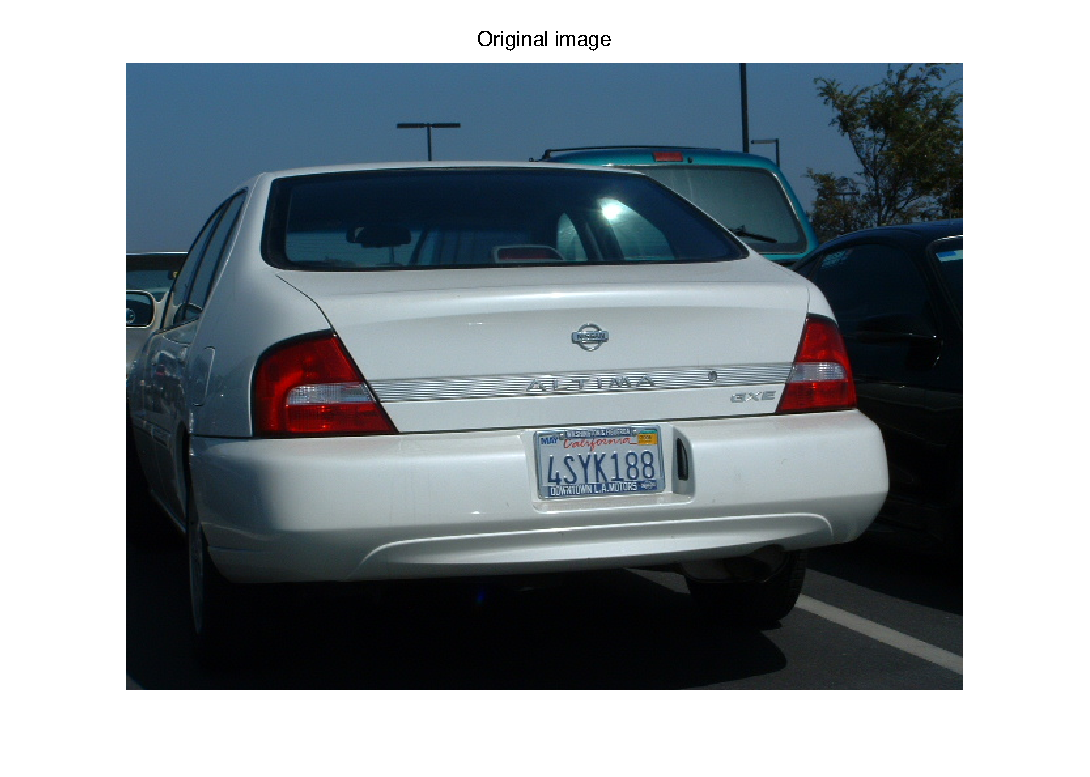
\includegraphics[width=5cm]{../report/img/cascader_original}
		}
		\subfigure{
			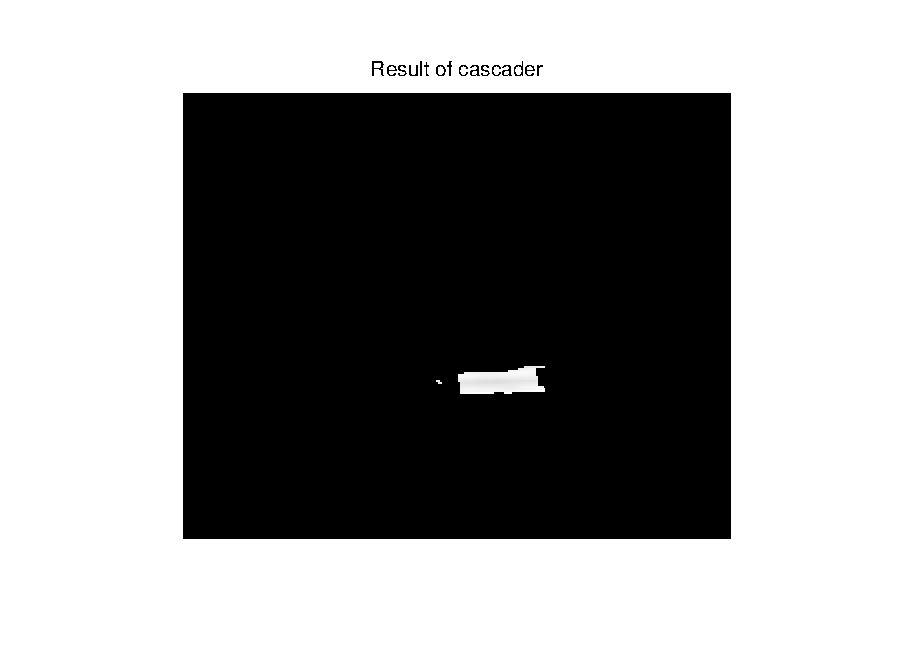
\includegraphics[width=5cm]{../report/img/cascader_result}
		}

	\end{figure}
}

\section{Conclusions}
\frame
{
  \frametitle{Conclusions}
	
  \begin{itemize}
  \item <+-| alert@+> xxx
  \end{itemize}
}
\end{document}
